%% This is an example file to show how to use JASA_manu.sty and related 
%% files written by Eric C. Anderson.  It's sort of a fly-by-night endeavor,
%% but I got it to work for me!!

\documentclass[11pt]{article}

\usepackage{graphicx}
\usepackage{float}
\usepackage{amssymb}
\usepackage{amsmath}

%% THE NEXT TWO LINES INSERT THE PACKAGES FOR JASA FORMAT:
\usepackage[default]{jasa_harvard}    % 	for formatting citations in text
\usepackage{JABES_manu}


%% CHANGING THE 'AND' IN THE HARVARD BIBLIOGRAPHY PACKAGE TO WHAT IT OUGHT TO BE
\renewcommand{\harvardand}{and}


%% A FEW NEWCOMMANDS FOR THE CONTENT IN THE EXAMPLE
%% NOT CRUCIAL TO THE USE OF JASA_manu.sty
\newcommand{\Dir}{\mathrm{Dir}}
\newcommand{\ceil}[1]{\lceil #1 \rceil}
\newcommand{\thh}{^\mathrm{th}}
\newcommand{\modtwo}{\mathrm{[mod~2]}}
\newcommand{\thetaof}[2]{\theta \langle #1;#2\rangle}
\newcommand{\Mpa}{M_\mathrm{P,A}}
\newcommand{\Ma}{M_\mathrm{A}}
\newcommand{\rjaccept}{\mathcal{A}}



%% Here is a hand-formatted bibliography reference list entry.
%% The command should be included in the NOTE field of the entry in the .bib file

\begin{document}



\title{Detecting Differential Expressed Genes in RNA-Seq Data \\ 
Accounting for Nuisance Covariates}
\author{Dan Nettleton  and Yet Nguyen\\
Department of Statistics \\ 
Iowa State University, Ames, IA 50010\\ 
email: \texttt{ntyet@iastate.edu} }

\maketitle


%% ABSTRACT

\newpage
\begin{center}
\textbf{Abstract}
\end{center}

Suppose that we have RNA sequencing (RNA-seq) read count data
on $J$ genes from an experiment with two treatment groups.
We want to find genes that are differentially expressed (DE) between
two treatment groups.
Analyses can often be complicated by the presence of nuisance factors
that arise due to experimental design limitations and heterogeneity of
experimental units that can be seen in  covariates
measured for each experimental unit and/or RNA sample. In this paper, we propose a method using QuasiSeq (Steve Lund et. al 2012) and backward selection strategy to obtain a  model for detecting DE genes between 2 treatment groups. 
There are 2 criteria using to do backward selection procedure. The first one is number of pvalue less than 0.05, denoted as pvalue05. The second one is the Cramer Von Mises statistics between Grenander Estimator of pvalue of each covariate to the uniform distribution, denoted as cvm. At each step of backward selection, the covariate has smallest value of pvalue05 (or cvm) is dropped, the procedure continue until the two group treatment is dropped. After this has been done, we have a set of models. The model has largest number of qvalue less than 0.05 among those will be pick up as final model for differential expressed analysis. We apply the method for detecting DE genes between 2 RFI Lines in RNA-Seq dataset in the presence of nuisance covariates such as Diet, RFI value, CBC covariate (neutrophil, lymphocyte, monocyte, eosinophil and basophil) and technical variables (processing batch, RNA concentration before and after globin depletion, RNA integrity number (RIN) before and after globin depletion
variables).



\vspace*{.3in}

\noindent\textsc{Keywords}: {Backward Selection, Grenander Estimator, qvalue, False Discovery Rate, Cramer Von Mises, RNA-Seq, Nuisance Covariates, Differential Expression.}

\newpage

\section{Introduction}
RNASeq data set is a $25320 \times 31$ table of count data corresponding
to 25320 genes of 31 pigs from 2 Lines: high RFI Line and low RFI
Line, and 2 Diets: high energy diet (Diet 1) and low energy diet (Diet
2). For Diet 1, the RNA data are from 7 low RFI line pigs and 8 high RFI
line pigs. For Diet 2, the RNA data are from 8 low RFI line pigs and 8
high RFI line pigs.
The number of genes analyzed is
12280. Those are genes with average counts greater than 8 and for
which there are at least four samples with non-zero counts.

\section{Methods}
Let $y_{ijk}$ is the count of gene $i$ from sample $j$ of treatment group $k$. Then suppose 
\[
y_{ijk} \sim NB(\mu_{ijk}, \omega_i), \log(\mu_{ijk}) = o_{jk} + Line*\beta_{line} + X_{(jk)}\beta,
\]

where $X$ is the desing matrix $31\times 23$ and $X_{(jk)}$ is the row of $X$ 
corresponding to sample $j$ of treatment group $k$, $\beta$ is the vector of parameter corresponding to  nuisance covariates.
\subsection{False Discovery Rate}
...............
\subsection{Grenander Estimator and Cramer Von Mises Statistics}
The Grenander (1956) density estimator is given by the slopes of the least concave majorant (LCM) of the empirical distribution function (ECDF). It is a decreasing piecewise-constant function and can be shown to be the non-parametric maximum likelihood estimate (NPMLE) under the assumption of a decreasing density (note that the ECDF is the NPMLE without this assumption). 

The Cramer-Von-Mises statistics is a criterion used for calculating the distance between  a cumulative distribution function $F^*$ compared to a given empirical distribution function $F_n$, or for comparing two empirical distributions. It is defined as

\[
\omega^2 = \int_{-\infty}^{\infty} [F_n(x)-F^*(x)]^2\,\mathrm{d}F^*(x) .
\]
.....................
\subsection{Backward Selection Procedure and Stopping Criteria}

Starting model includes all covariates of interest. For each covariate,
we conduct a Likelihood Ratio Test using QuasiSeq of the full model
vs. the reduced model obtained from the full model by deleting the
considered covariate. We collect the set of pvalues of all genes from
the tests.
Obtain the number of genes with pvalues less than or equal 0.05 (This is the criterion named pvalue05).
Obtain Grenander CDF estimator of the empirical CDF of the sample
from those pvalues.
Obtain Craḿer-Von-Mises statistics,
 statistics between the Grenander CDF and
uniform(0,1) CDF.
Exclude the covariate corresponding to the smallest value in each criterion.

The procedure will be terminated until the Line effect is excluded.  Then the final model will be used for differential expression analysis will be the model which has largest number of pvalue of Line effect less than 0.05.
\section{Real Data Analysis}
\begin{figure}[h!]
\centering
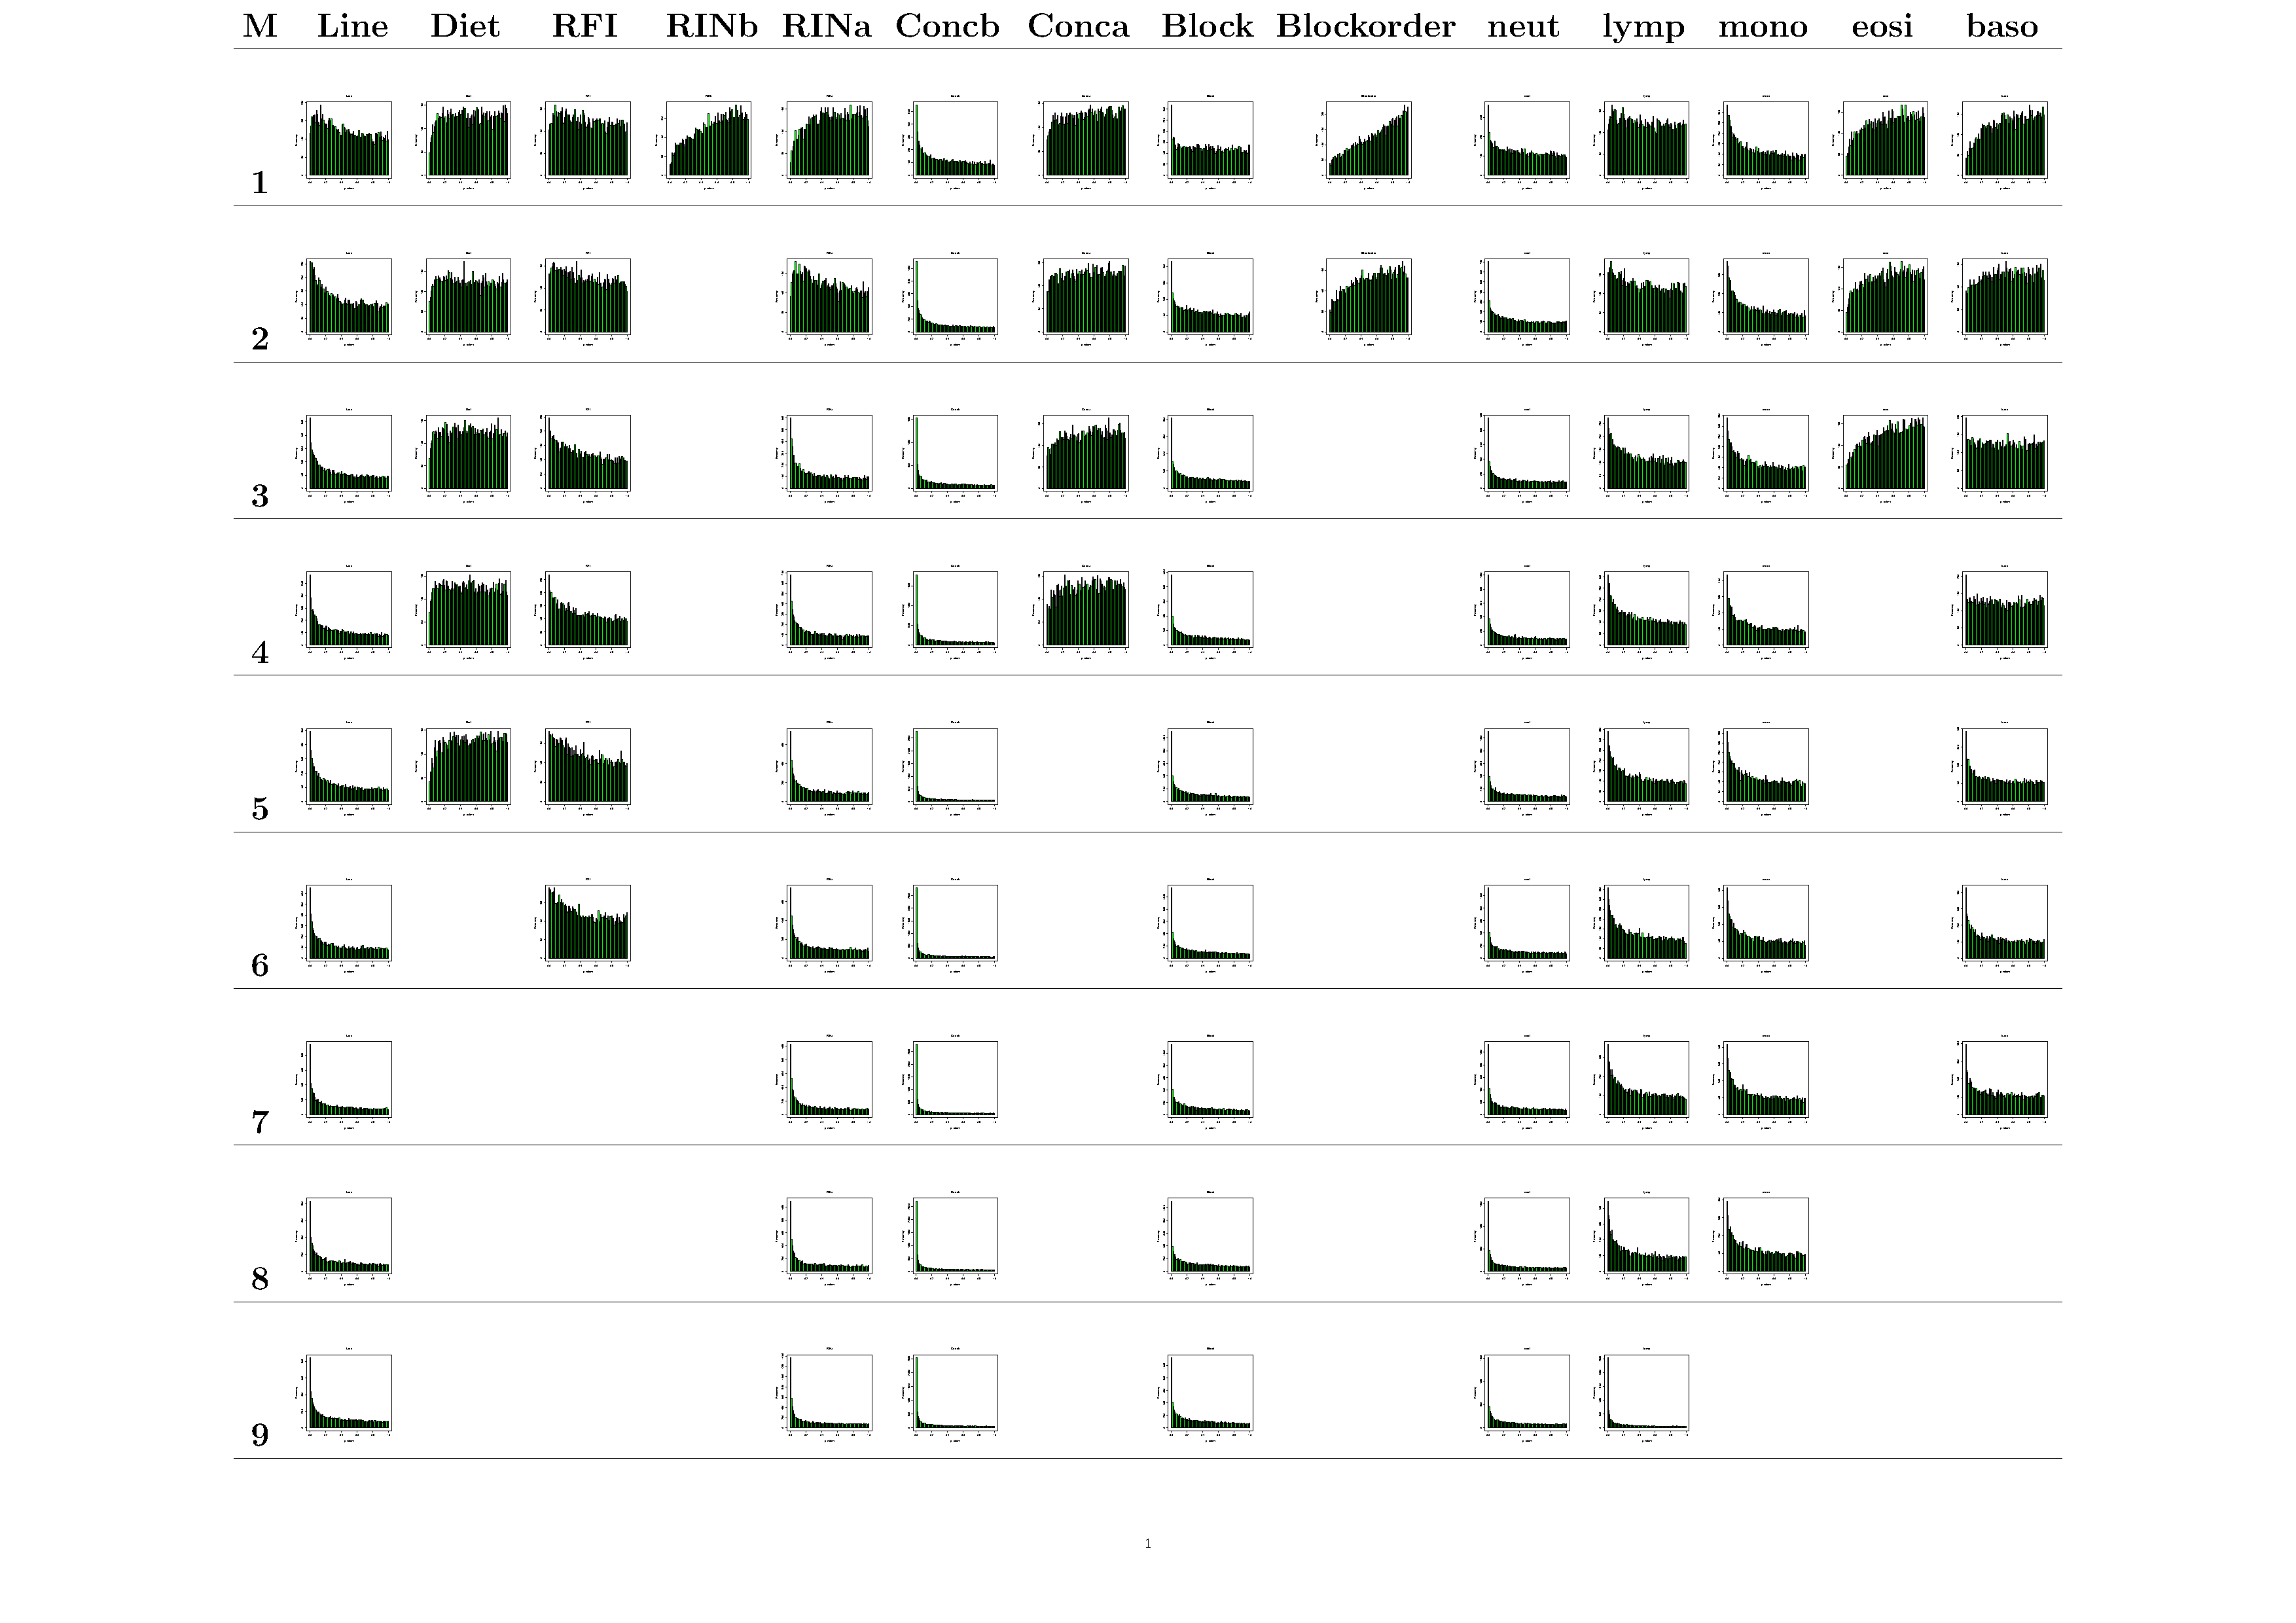
\includegraphics[scale = 0.23]{PlotG9P2PairedEndCBCpvalue05.pdf}
\caption{Backward Modelselection for RFI data using the criterion based on number of pvalue less than 0.05 in each step of excluding one covariate. }
\end{figure}

\section{Simulation Justification based on Real Data}

\section*{Acknowledgments}
% This material is based upon work supported by Agriculture and Food
% Research Initiative Competitive Grant No. 2011-68004-30336 from
% the USDA National Institute of Food and Agriculture, and the
% National Science Foundation (NSF) under Grant No. 0922746.
% Any opinions, findings, and conclusions or recommendations expressed
% in this material are those of the authors and do not necessarily reflect
% the views of the USDA or NSF.

%% HERE WE DECLARE THE BIBLIOGRAPHYSTYLE TO USE AND THE BIBLIOGRAPHY DATABASE

\end{document}